\chapter{Arpeggiator \& Step Sequencer}
\label{arpeggiator}

\begin{center}
    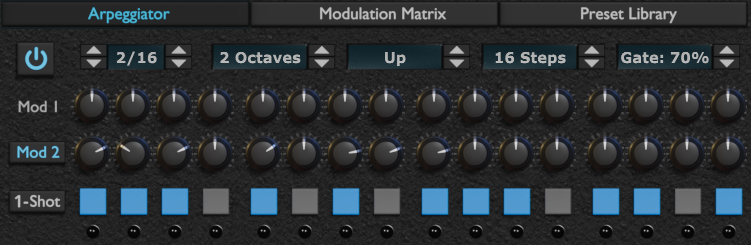
\includegraphics[width=\textwidth]{graphics/arpeggiator.png}
\end{center}

The Arpeggiator \& Step Sequencer is a tool which is able to automatically play complex rhythmic sequences from a given set of input notes. Activating this module overrides the notes you're inputting into the synthesizer and generates note sequences itself.

\begin{tcolorbox}[colback=yellow!10!white,
    colframe=white!20!black,
    center,
    valign=top,
    halign=left,
    center title,
    width=\textwidth]

    The Arpeggiator \& Step Sequencer occupies the same space in the GUI as the modulation matrix and the Preset Library. If you can't locate the module in the lower right corner of the GUI, press the "Arpeggiator" button above the modulation matrix:

    \begin{center}
        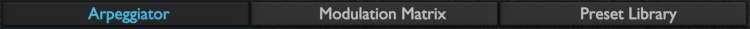
\includegraphics[width=\textwidth]{graphics/arpeggiator_button.png}
    \end{center}
\end{tcolorbox}

The basic operation of this module is to listen for the inputs you play on the keyboard and play them over a set of octaves. You can control various parameters, like the amount of octaves, the direction of the arpeggio, gate length, which notes to omit and many more.

\audioparameter{Arpeggiator On}{0}{1}{
    \begin{center}
        
\includegraphics[height=0.08\textwidth]{graphics/arpeggiator_on.png}
    \end{center}    

    Turns the Arpeggiator \& Step Sequencer module on or off.
}

\audioparameter{Arpeggiator Step Time}{1}{0}{
    \begin{center}
        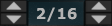
\includegraphics[width=0.17\textwidth]{graphics/arpeggiator_speed.png}
    \end{center}
    Controls the time one step takes, synced to the host BPM. The image above represents a length of $2/16$th or $1/8$th note. This parameter can be modulated in the \modmatrix to achieve non-synced values.
}

\audioparameter{Arpeggiator Octaves}{0}{0}{
    \begin{center}
        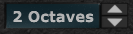
\includegraphics[width=0.17\textwidth]{graphics/arpeggiator_octaves.png}
    \end{center}
    Controls over how many octaves the arpeggio will be played. For a pure Step Sequencer style operation, set this value to 1.
}

\audioparameter{Arpeggiator Gate Length}{1}{0}{
    \begin{center}
        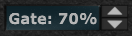
\includegraphics[width=0.17\textwidth]{graphics/arpeggiator_gate.png}
    \end{center}
    Controls how long a note is played, before a note-off signal is sent to the synthesizer. The times are represented in percent of the current step time. If the gate length is bigger than 100\%, each step will overlap into the next step.
}


\audioparameter{Arpeggiator Direction}{0}{0}{
    \begin{center}
        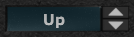
\includegraphics[width=0.17\textwidth]{graphics/arpeggiator_direction.png}
    \end{center}

    Determines the play style of the arpeggiator. The resulting notes for the various directions will be displayed here for "Arpeggiator Octaves" set to 2, Speed of $1/16$ and a C-major chord as an input:

    \begin{center}
        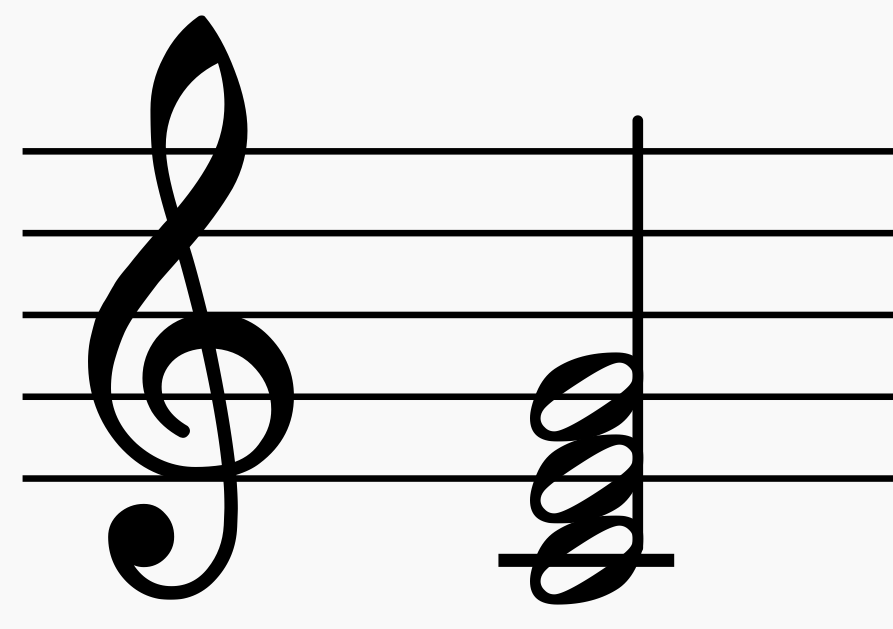
\includegraphics[height=0.08\textwidth]{graphics/c_major.png}
    \end{center}

    \fat{Direction: Up}
    \begin{center}
        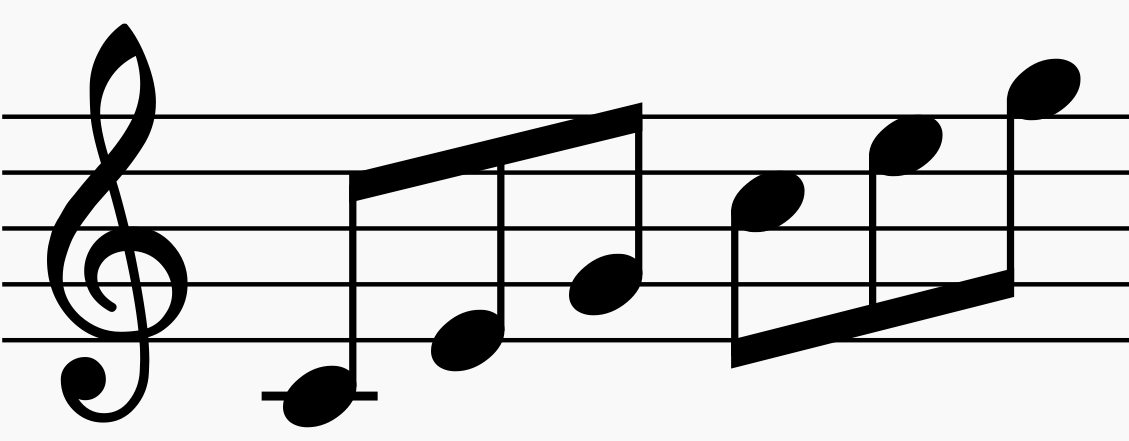
\includegraphics[height=0.08\textwidth]{graphics/arpeggiator_up.png}
    \end{center}

    \fat{Direction: Down}
    \begin{center}
        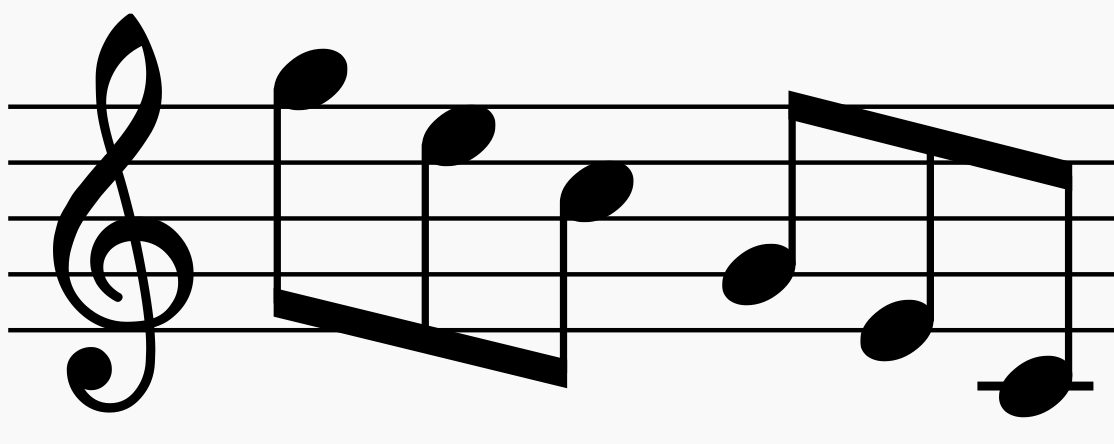
\includegraphics[height=0.08\textwidth]{graphics/arpeggiator_down.png}
    \end{center}

    \fat{Direction: Up Down}
    \begin{center}
        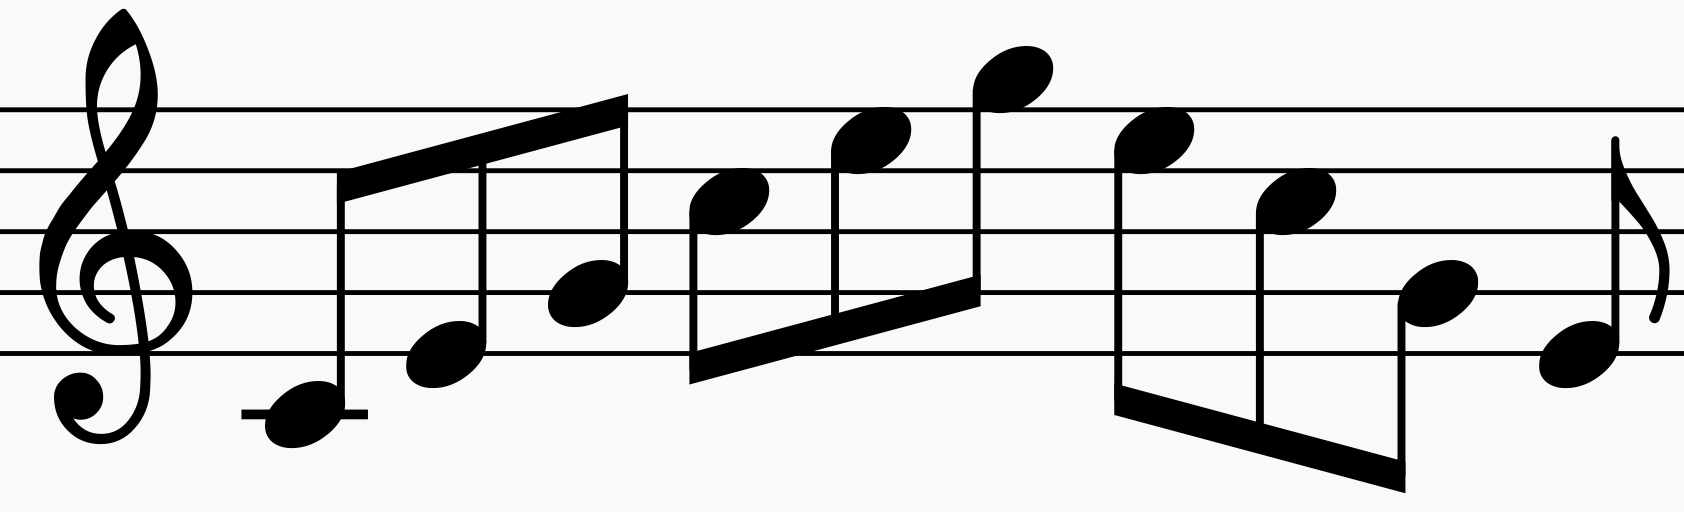
\includegraphics[height=0.08\textwidth]{graphics/arpeggiator_updown.png}
    \end{center}

    \fat{Direction: Down Up}
    \begin{center}
        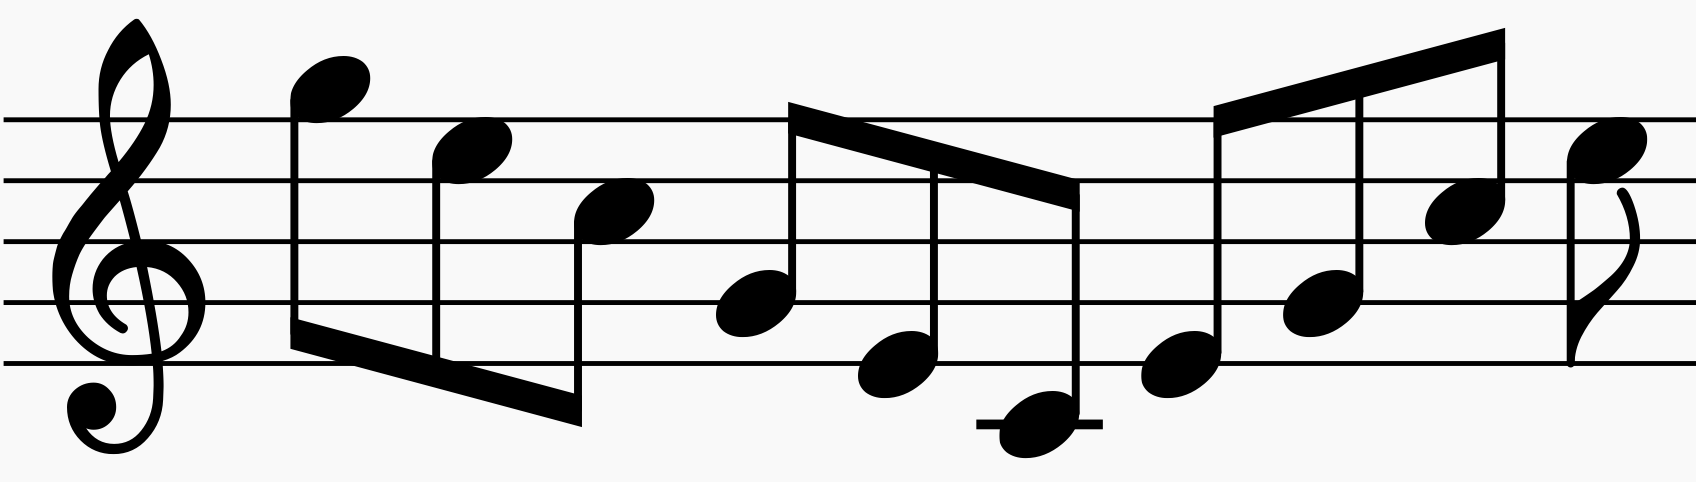
\includegraphics[height=0.08\textwidth]{graphics/arpeggiator_downup.png}
    \end{center}

    \fat{Direction: Crawl Up}
    \begin{center}
        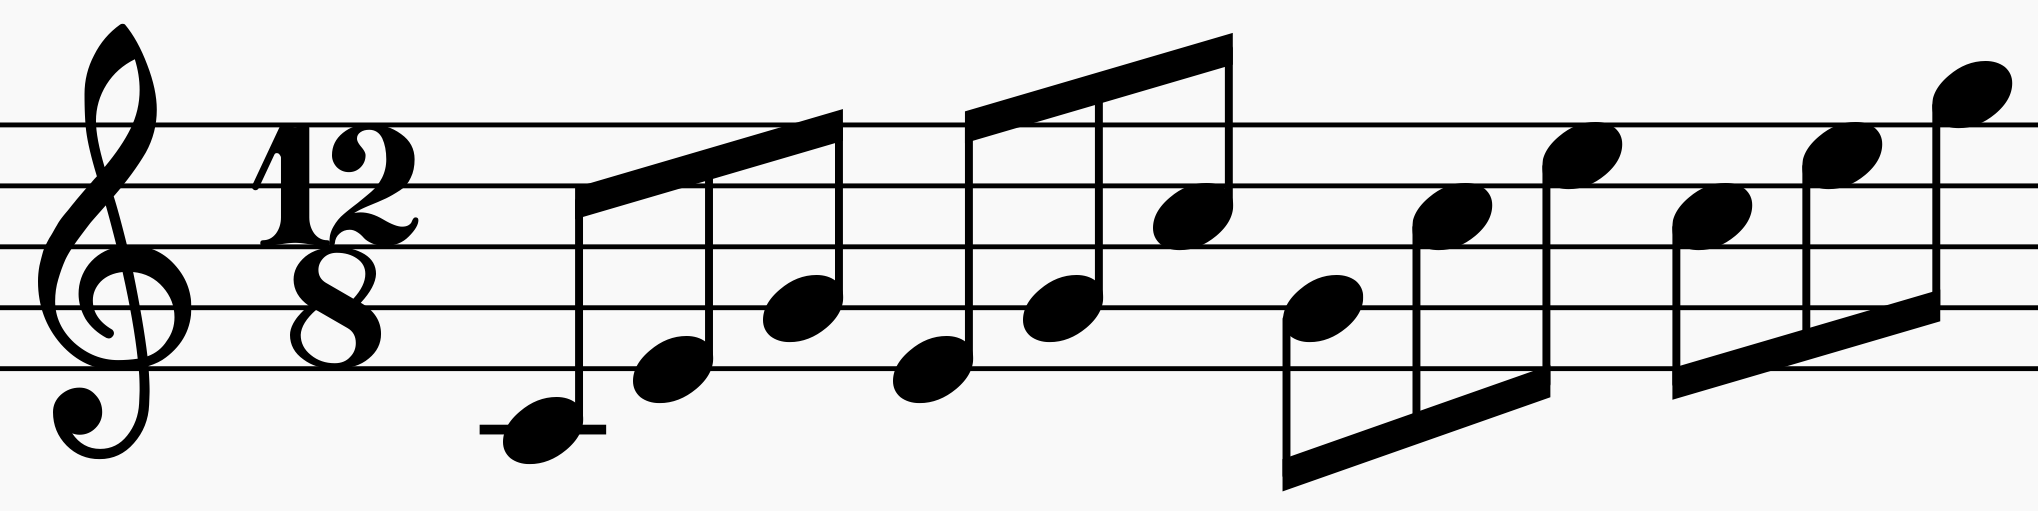
\includegraphics[height=0.08\textwidth]{graphics/arpeggiator_crawlup.png}
    \end{center}

    \fat{Direction: Crawl Down}
    \begin{center}
        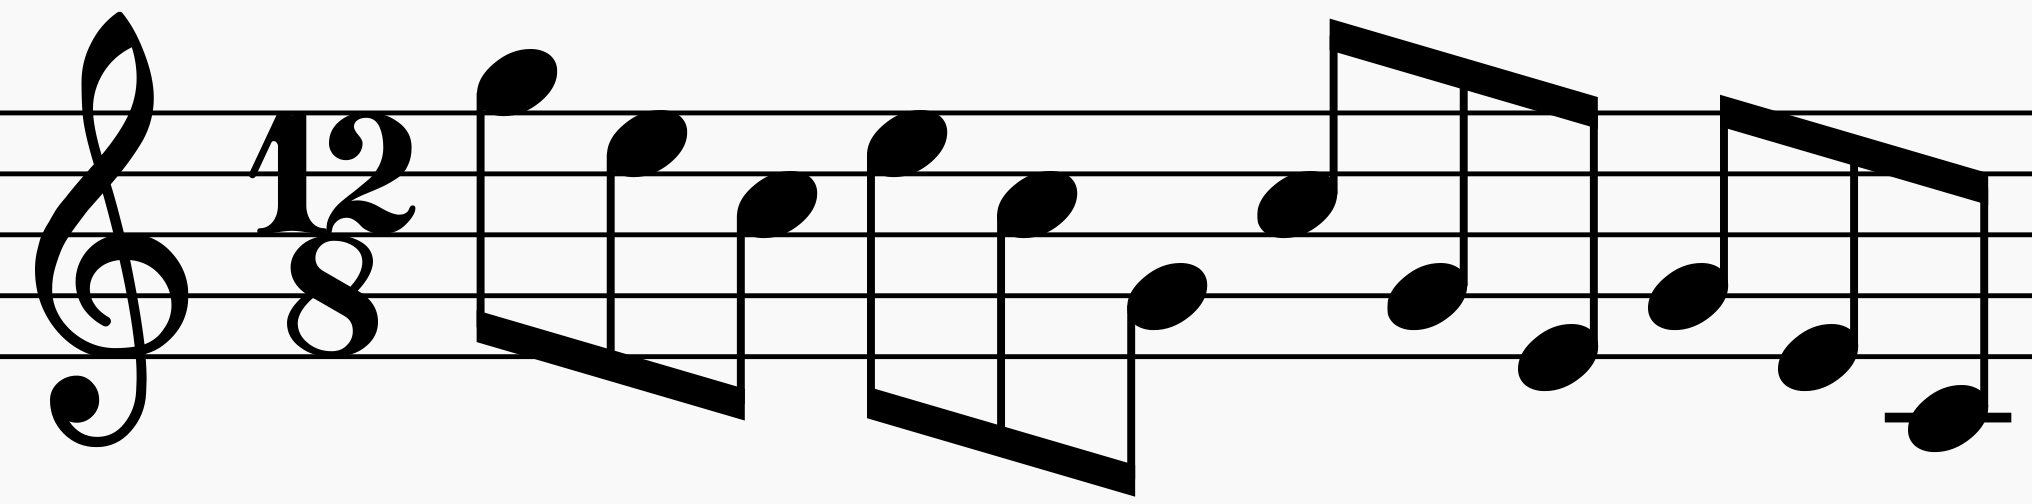
\includegraphics[height=0.08\textwidth]{graphics/arpeggiator_crawldown.png}
    \end{center}

}

\audioparameter{Step Active}{0}{0}{
    \begin{center}
        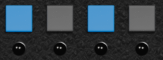
\includegraphics[height=0.08\textwidth]{graphics/arpeggiator_step_on.png}
    \end{center}

    Turns a step in the sequence on or off. This can be used to easily create rhytmic patterns.
}

\audioparameter{Arpeggiator Steps}{0}{0}{
    \begin{center}
        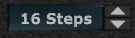
\includegraphics[height=0.05\textwidth]{graphics/arpeggiator_steps.png}
    \end{center}

    Limits the number of steps to be played before the sequence wraps around.

    To clarify: "Sequence" here does not mean the note-pattern created by the arpeggiator. Rather it means the rhythmic pattern created by enabling or disabling steps with the "Step Active" buttons. You can tell the current sequence size by the amount of LEDs which are displayed on the bottom of the module.

    If the sequence has ended, it will either start over, or stop, depending on the parameter "One-Shot".
}

\audioparameter{Arpeggiator One-Shot}{0}{1}{
    Enables one-shot mode: In one-shot mode, the sequence is stopped after playing through it once.

    To clarify: "Sequence" here does not mean the note-pattern created by the arpeggiator, but the sequence length as set by the parameter "Arpeggiator Steps". You can tell the current sequence size by the amount of LEDs which are displayed on the bottom of the module.
}

\audioparameter{Arpeggiator Modulation 1}{0}{1}{
    \begin{center}
        
\includegraphics[height=0.05\textwidth]{graphics/arpeggiator_mod1.png}
    \end{center}

    A set of freely definable modulation values. This value will be transmitted to the note that is triggered from this step in the sequence, and can be used in the \modmatrix via the modulation source "Arp Mod 1".

    This can be used to bring movement into the sequence by modulating sound parameters as the sequence progresses.
}

\begin{tcolorbox}[colback=yellow!10!white,
    colframe=white!20!black,
    center,
    valign=top,
    halign=left,
    center title,
    width=\textwidth]

    The second row of knobs in the Arpeggiator \& Step Sequencer can be toggled to either be "Arpeggiator Modulation 2" or "Arpeggiator Transpose" by the button to the left:

    \begin{center}
        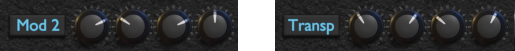
\includegraphics[width=0.6\textwidth]{graphics/arpeggiator_mod_vs_transpose.png}
    \end{center}

    Both functionalities will be available at the same time, but only one set of knobs is visible.
\end{tcolorbox}

\audioparameter{Arpeggiator Modulation 2}{0}{1}{
    \begin{center}
        
\includegraphics[height=0.05\textwidth]{graphics/arpeggiator_mod2.png}
    \end{center}

    A set of freely definable modulation values. This value will be transmitted to the note that is triggered from this step in the sequence, and can be used in the \modmatrix via the modulation source "Arp Mod 2".

    This can be used to bring movement into the sequence by modulating sound parameters as the sequence progresses.

    \vspace{3mm}
    Make sure the button to the left of the second row is set to "Mod 2" and not "Transp" to access these parameters.
}

\audioparameter{Arpeggiator Transpose}{0}{1}{
    \begin{center}
        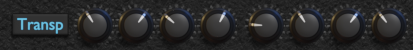
\includegraphics[height=0.05\textwidth]{graphics/arpeggiator_transp.png}
    \end{center}

    Transposes the corresponding step in the sequence in semitones. 
    
    When used with a "Arp Octaves" set to one and only one key played, this can be used to create custom note sequences.

    \vspace{3mm}
    Make sure the button to the left of the second row is set to "Transp" and not "Mod" to access these parameters.
}
